\section{Xwindow Interface}
\markright{\arabic{section}. Xwindow}
The Xwindow interface on EusLisp becomes available when EusLisp is
invoked by the name of {\tt 'eusx'}.
\footnote{Eusx is a symbolic link to eus.}
The "DISPLAY" environment variable should be properly set to your Xserver,
since eusx tries to connect to Xserver referencing
the "DISPLAY" environment variable when it starts up.

EusLisp defines three levels of xwindow interface:
(1) Xlib functions, (2) Xlib classes, and (3) XToolKit classes.
All the xwindow functions described in this section and the following
XToolKit section are contained in the "X" package.
The function names of the original Xlib are changed so that
all constituent letters are converted to upcase
and the first 'X' prefix is removed.
For example, {\tt XdefaultGC} is named {\tt X:DEFAULTGC},
not {\tt X:XDEFAULTGC}.

The Xlib functions are defined as foreign functions
as the lowest level interface to Xwindow system.
These Xlib functions should be used carefully, 
since parameter type check or parameter number check is not performed.
For an instance, all the Xlib call requests {\tt x:*display*} argument
to identify the connection to Xserver, and if you forget it, Xlib reports
an error and the process dies.
The second level interface, Xlib classes are provided
to avoid this inconvenience and to make the interface object-oriented.
%By instantiating the xwindow class, you will get a window on a screen,
%and sending messages to the instance, you can draw lines, strings, or whatever
%in it.
This section focuses on this second level interface.
Even higher level xwindow library called XToolKit is explained 
in the next section.

Classes described in this section have the following inheritance
hierarchy.

\begin{quote}
\begin{verbatim}
propertied-object
   viewsurface
      x:xobject
         x:gcontext
         x:xdrawable
             x:xpixmap
             x:xwindow
   colormap
\end{verbatim}
\end{quote}

\subsection{\label{xvariables}Xlib global variables and misc functions}
\begin{refdesc}
\vardesc{x:*display*}{X's display ID (integer).}
\vardesc{x:*root*}{default root window object. }
\vardesc{x:*screen*}{default screen ID (integer).}
\vardesc{x:*visual*}{default visual ID (integer).}
\vardesc{x:*blackpixel*}{black pixel = 1}
\vardesc{x:*whitepixel*}{white pixel = 0}
\vardesc{x:*fg-pixel*}{default foreground pixel referenced at window creation,
normally {\tt *blackpixel*}.}
\vardesc{x:*bg-pixel*}{background pixel referenced at window creation,
normally {\tt *whitepixel*}}
\vardesc{x:*color-map*}{the system's default color-map}
\vardesc{x:*defaultGC*}{the default gcontext referenced at pixmap creation.}
\vardesc{x:*whitegc*}{GC whose foreground color is white.}
\vardesc{x:*blackgc*}{GC whose foreground color is black.}

% \vardesc{*gray-gc*}{half-tone GC}
\vardesc{*gray-pixmap*}{the result of {\tt (make-gray-pixmap 0.5)}}
\vardesc{*gray25-pixmap*}{16x16 pixmap,
a quarter of pixels are {\tt *fg-pixel*} and three quarters {\tt *bg-pixel*}.}
\vardesc{*gray50-pixmap*}{16x16 pixmap, a half of pixels are {\tt *fg-pixel*}.}
\vardesc{*gray75-pixmap*}{16x16 pixmap, three quarters of pixels are black.}
\vardesc{*gray25-gc*}{25\% gray GC made from  {\tt *gray25-pixmap*}.}
\vardesc{*gray50-gc*}{50\% gray GC made from  {\tt *gray50-pixmap*}.}
\vardesc{*gray75-gc*}{75\% gray GC made from  {\tt *gray75-pixmap*}.}
\vardesc{*gray*}{{\tt "\#b0b0b0"}}
\vardesc{*bisque1*}{{\tt "\#ffe4c4"}}
\vardesc{*bisque2*}{{\tt "\#eed5b7"}}
\vardesc{*bisque3*}{{\tt "\#cdb79e"}}
\vardesc{*lightblue2*}{{\tt "\#b2dfee"}}
\vardesc{*lightpink1*}{{\tt "\#ffaeb9"}}
\vardesc{*maroon*}{{\tt "\#b03060"}}
\vardesc{*max-intensity*}{65535}
\vardesc{font-cour8}{{\tt (font-id "*-courier-medium-r-*-8-*")}}
\vardesc{font-cour10}{{\tt (font-id "*-courier-medium-r-*-10-*")}}
\vardesc{font-cour12}{{\tt (font-id "*-courier-medium-r-*-12-*")}}
\vardesc{font-cour14}{{\tt (font-id "*-courier-medium-r-*-14-*")}}
\vardesc{font-cour18}{{\tt (font-id "*-courier-medium-r-*-18-*")}}
\vardesc{font-courb12}{{\tt (font-id "*-courier-bold-r-*-12-*")}}
\vardesc{font-courb14}{{\tt (font-id "*-courier-bold-r-*-14-*")}}
\vardesc{font-courb18}{{\tt (font-id "*-courier-bold-r-*-18-*")}}
\vardesc{font-helvetica-12}{{\tt (font-id "*-Helvetica-Medium-R-Normal-*-12-*")}}
\vardesc{font-lucidasans-bold-12}{{\tt (font-id "lucidasans-bold-12")}}
\vardesc{font-lucidasans-bold-14}{{\tt (font-id "lucidasans-bold-14")}}
\vardesc{font-helvetica-bold-12}{{\tt (font-id "*-Helvetica-Bold-R-Normal-*-12-*")}}
\vardesc{font-a14}{{\tt (font-id "*-fixed-medium-r-normal-*-14-*")}}

%\vardesc{x:*reversevideo*}{}
\vardesc{x:*xwindows*}{a list of all windows including subwindows
created and maintained by EusLisp.}
\vardesc{x:*xwindow-hash-tab*}{a hash table to look up the xwindow object
by its drawable ID.
In the event structure obtained by {\tt x:nextevent} is a window ID,
and {\tt x:window-main-loop} calls {\tt x:event-window} to know
the corresponding xwindow object using this table.}
%\vardesc{x:gcval}{}

\funcdesc{xflush}{}{
sends all commands retained in the Xlib command buffer to Xserver.
Since Xlib buffers output to Xserver,
commands you issued commands to Xserver are not executed immediately.
This is necessary to decrease network traffic and the frequency
of process switching.
To flush the command buffer to see the effects of the commands,
use {\bf xflush} or send {\bf :flush}
message to  xwindow objects.
}
\funcdesc{find-xwindow}{subname}{
Each xwindow may have name specified at the creation time.
Find-xwindow looks in the *xwindows* list and returns a list
of windows that have 'subname' as a substring
of its name. }

\end{refdesc}

\subsection{Xwindow}

\begin{refdesc}

\classdesc{Xobject}{geometry:viewsurface}{}{
The common super class for all the Xwindow related classes.
Currently, no slots variables and methods are defined.}

\classdesc{Xdrawable}{Xobject}
{(drawable  \hspace{10mm} \=  ; drawable  ID \\
 \> gcon \>  ; this drawable's default graphic context object\\
\> bg-color \> ; background color \\
\> width height \> ; horizontal and vertical dimensions in dots}
{{\bf Xdrawable} defines rectangular regions where graphics objects such as
lines and strings can be drawn.
{\bf Xdrawable} is an abstract class to define
common methods for xwindow and xpixmap,
and instantiation of this class has no effect.}

\methoddesc{:init}{id}{
{\em Id} is set to the {\em drawable} slot as the ID of this drawable.
A new GC (graphic context) is created and set to {\em gcon} as 
the default GC of this drawable object.}
\methoddesc{:drawable}{}{returns drawable id.}
\methoddesc{:flush}{}{flushes commands retained in the Xlib's buffer.}
\methoddesc{:geometry}{}{
returns the list of seven geometric attributes,
{\em root-window-id, x-position, y-position,
width, height, border-width} and {\em visual's depth}.}
\methoddesc{:height}{}{
returns the height (dots in y direction) of this drawable.}
\methoddesc{:width}{}{
returns width (dots in x direction) of this drawable.}
\methoddesc{:gc}{\&rest newgc}{
If no {\em newgc} is given, the current gc object is returned.
If {\em newgc} is an instance of gcontext,
it is set to the gc of this drawable.
Otherwise, {\em newgc} is regarded as a message and  sent to
the current gc.}
\methoddesc{:pos}{}{returns an integer vector representing 
the position of this drawable.
The position is always defined relative to the 
parent window, and windows created as direct subwindows of the root
window under the intervention of the window manager return the constant
coordinates in their surrounding title window regardless to their
true position in the root.}
\methoddesc{:x}{}{returns the {\em x} coordinate of this drawable relatively to
the parent window.}
\methoddesc{:y}{}{returns the {\em y} coordinate of this drawable relatively to
the parent window.}

\methoddesc{:copy-from}{drw}{
{\em Drw} is another drawable object (xwindow or pixmap).
The contents of {\em drw} is copied to this drawable.}

\begin{figure}
\begin{center}
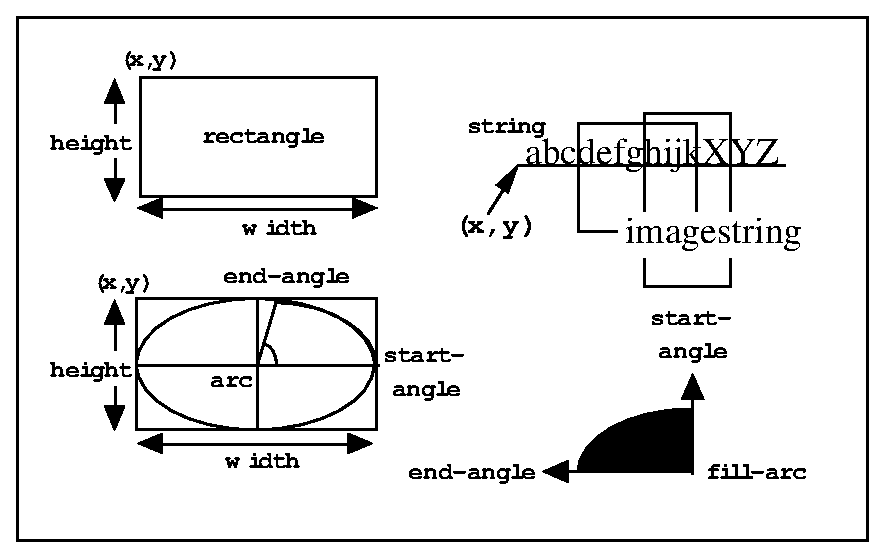
\includegraphics[height=6cm]{fig/xdraw.ps}
%\epsfile{file=fig/xdraw.ps,height=6cm}
%\mbox{
%\epsfysize=6cm
%\epsfbox{fig/xdraw.ps}
%}
\end{center}
\caption{drawing primitives\label{xdraw}}
\end{figure}


\methoddesc{:point}{x y \&optional (gc gccon)}{
draws a point at $(x, y)$ with optional {\em gc}.}
\methoddesc{:line}{x1 y1 x2 y2 \&optional (gc gcon)}{
draw a line from {\em (x1, y1)} to {\em (x2, y2)}
with optional {\em gc}. {\em x1, y1, x2,} and{\em y2} must be integers.}
\methoddesc{:rectangle}{x y width height \&optional (gc gcon)}{
draws a rectangle whose center is located at {\em (x, y)}
and size is specified by {\em width} and {\em height}.}
\methoddesc{:arc}{x y width height angle1 angle2 \&optional (gc gcon)}{
draws an elliptic arc whose center is {\em (x, y)} and starting angle at 
{\em angle1} and ending angle at {\em angle2}.
Angles should be given by radian.}
\methoddesc{:fill-rectangle}{x y width height \&optional (gc gcon)}{
fills in a rectangular region.}

\methoddesc{:fill-arc}{x y width height angle1 angle2 \&optional (gc gcon)}{
fills in an arc.
}
\methoddesc{:string}{x y str \&optional (gc gcon)}{
displays the string {\em str} starting at {\em (x, y)}. The background is
not filled.}
\methoddesc{:image-string}{x y str \&optional (gc gcon)}{
displays an imagestring of {\em str}. Imagestring fills background.}
\methoddesc{:getimage}{\&key x y width height (mask \#ffffffff) (format 2)}{
gets ximage from the server and returns the pixel data in a string.
The pixel data sent from the server is once stored in Xlib's ximage structure,
then copied to the string row by row.
The ximage structure is automatically destroyed.
The image string obtained by {\tt :getimage} can be used to make
a {\tt pixel-image}, which can be written to a file in the pbm formats
as described in section \ref{PBMfile}.}
\methoddesc{:putimage}{image \&key src-x src-y dst-x dst-y width height ((:gc g) gc)}{
puts {\em image} to the specified location in this drawable.
{\em image} is a string or a address pointing to an ximage structure.}
\methoddesc{:draw-line}{from to}{
is same as {\bf :line} method,
and provided for the compatibility with other viewsurface classes.}
\methoddesc{:line-width}{\&optional dots}{sets line-width of this drawable's
default GC. Use of the {\tt :gc :line-width} message is recommended.}
\methoddesc{:line-style}{\&optional dash}{sets line-style of this drawable's
default GC. Use of the {\tt :gc :line-style} is preferable.}
\methoddesc{:color}{\&optional c}{sets color of this drawable.}
%\methoddesc{:set-show-mode}{}{
%sets copy mode. this function usually uses for monochrome display.}
%\methoddesc{:set-erase-mode}{}{
%sets erase mode. this function usually uses for monochrome display.}
%\methoddesc{:set-xor-mode}{}{
%sets xor mode. this function usually uses for monochrome display.}
\methoddesc{:clear}{}{
clears full screen. this method calls {\tt :clear-area}}
\methoddesc{:clear-area}{\&key :x  :y :width :height :gc}{
clears a rectangle using the {\tt :fill-rectangle} method.}

\classdesc{Xpixmap}{Xdrawable}{}{Pixmap is a drawable that is often used
as a picture buffer or a background pattern.
Unlike xwindow, pixmap itself is not visible until it is copied to xwindow
or pixmap does not generate any event.}

\methoddesc{:init}{id}{initializes this pixmap.}
\methoddesc{:create}{\&key (width 500) (height 500) (depth 1) (gc *defaultgc*)}{
creates a {\em width} x {\em height} pixmap with {\em gc} as its
default GC.}
\methoddesc{:create-from-bitmap-file}{fname}{
creates a pixmap from a bitmap file.}
\methoddesc{:write-to-bitmap-file}{fname}{
writes the contents of this pixmap into a bitmap file,
which can be read back to create a pixmap by {\bf :create-from-bitmap-file}
method.}
\methoddesc{:destroy}{}{
destroys this pixmap and frees X resources.}

%%%%%% X W I N D O W
\classdesc{Xwindow}{Xdrawable}{(parent subwindows backing-pixmap event-forward)
}{{\bf Xwindow} defines visible rectangular regions of the screen.
It is inherited not only by {\bfx text-window} and {\bf canvas} where
any graphics objects can be drawn, but also by many {\bf panel-items}
and {\bf scroll-bars}, which look like graphics objects rather than windows.}

\longdescription{:create}{\&key ( \= (:parent *root*) \` [method] \\
\> (x 0) (y 0) (size 256) (width size) (height size) (border-width 2) \\
\> (save-under nil) (backing-store :always) (backing-pixmap nil)\\
\> (border *fg-pixel*) (background *bg-pixel*) \\
\> (map T) (gravity :northwest) \\
\> (title "WINDOW") (name title) \\
\> (font) \\
\> event-mask (:key :button :enterLeave :configure :motion)}
{creates and initializes a xwindow.
When {\em parent} is given, this window is created as a subwindow
of {\em parent}, and is registered in the {\em subwindows} list of
the {\em parent}.
{\em X, y, size, width, height} and {\em border-width} determine
the location and the dimensions of this window.
{\em Save-under} and {\em backing-store} control the Xserver's behaviors
taken upon when the window is re-mapped. {\em Save-under} is either
T or NIL, while {\em backing-store} is either {\tt :notUseful, :WhenMapped},
or {\em :Always}.
When {\em backing-pixmap} is T, a pixmap of the same size as this window
is created by EusLisp, and maintained as a backing-store in case
the Xserver does not have the capability of backing-store.
{\em Border} and {\em background} specify the {\em border\_pixel}
and {\em background\_pixel} attributes, respectively.
{\em Map} should be set NIL, if this window should not appear
immediately after its creation, as is the case many small windows 
are created as panel-buttons in a {\bf panel}.
{\em Title} is the window title which appears in the title bar of 
the window.
{\em Name} is the name of the window stored in the property-list
of this xwindow object and printed by the printer.
X's events reported to this window are determined by 
{\em Event-mask}, that is, either an integer representing a bit-coded event-mask
or a list of the following symbols:
{\tt :key, :button, :enterLeave, :motion} and {\tt :configure}.
If more precise control is needed, the following symbols for each event
can be specified: {\em :keyPress, :keyRelease, :ButtonPress, :ButtonRelease,
:EnterWindow, :LeaveWindow, :PointerMotion, :PointerMotionHint, 
:ButtonMotion, :KeyMapState, :Exposure, :VisibilityChange, :StructureNotify,
:ResezeRedirect, :SubstructureNotify, :SubstructureRedirect,
:FocusChange, :PropertyChange, :ColormapChange} and {\tt :OwnerGrabButton}.
{\tt :Key} enables both {\tt :keyPress} and {\tt :KeyRelease}, and
{\tt :button} enables both {\tt :ButtonPress} and {\tt :ButtonRelease}.
When an event is sent from the server, {\bfx window-main-loop} analyzes
the event structure and send the {\tt :KeyPress, :KeyRelease, :buttonPress,
:ButtonRelease, :EnterNotify, :LeaveNotify, :MotionNotify, :ConfigureNotify}
message to the window where the event occurred.}

\methoddesc{:map}{}{makes this xwindow and all the subwindows visible.}
\methoddesc{:unmap}{}{makes this xwindow and all the subwindows invisible.}
\methoddesc{:selectinput}{event-mask}{
{\em Event-mask} is either an integer or a list of eventmask symbols.
Each event corresponding to the bit turned-on or 
enumerated in the {\em event-mask} list
becomes to be reported to this window.}
\methoddesc{:destroy}{}{destroys this xwindow and frees X resource.
The corresponding entries in {\tt *xwindows*} and {\tt *xwindow-hash-tab*}
are also deleted so that this window object could be garbage-collected.
All subwindows are also deleted by sending {\tt :destroy}.
This window is dissociated from the subwindow list of the parent window.
The {\em drawable} ID is set to NIL.}
\methoddesc{:parent}{}{returns the parent window object.}
\methoddesc{:subwindows}{}{
returns the list of all the subwindows.
The subwindow most recently created comes first in the list.
Only the direct subwindows of this window are listed and
subwindows of the subwindows are not.}
\methoddesc{:associate}{child}{register the {\em child} window
as a subwindow of this window.}
\methoddesc{:dissociate}{child}{removes the {\em child} window
of the {\em subwindows} list.}

%\methoddesc{:save}{}{
%copies the content of this window to the backing-store pixmap.}
%\methoddesc{:refresh}{}{
%copies from the backing-store.}

\methoddesc{:title}{title}{
changes the title of this window.
Though the title is in the Xserver, it is maintained and displayed by
the window manager.}

\methoddesc{:attributes}{}{returns an integer-vector representing
the attributes of this window.}
\methoddesc{:visual}{}{returns the visual resource id for this window.} 
\methoddesc{:screen}{}{returns the screen resource id for this window.} 
\methoddesc{:root}{}{returns the root window id.} 
\methoddesc{:location}{}{
returns a two dimensional integer-vector describing the x and y coordinates
of this window.}
\methoddesc{:depth}{}{returns the depth (number of color planes) of this window.}
\methoddesc{:size}{}{returns the size (width and height) of this window.}
\methoddesc{:colormap}{}{returns colormap resource id for this window.} 

\methoddesc{:move}{newx newy}{
changes the location of this window to {\em (newx, newy)}.
The coordinates are given relative to the parent window.}
\methoddesc{:resize}{width height}{
changes the size of this window.
Probably because the size parameters are cached in the Xlib on the client side,
{\tt :geometry} message immediately after {\tt :resize} may return wrong (old)
result.}
\methoddesc{:raise}{}{brings this window upfront.}
\methoddesc{:lower}{}{pushes this window to the back.}
\methoddesc{:background}{pixel}{changes the background pixel value (the
index in the color map) to {\em pixel}.
The {\em pixel} value is also stored in the {\em bg-color} slot.
{\tt :Clear} operation is performed to fill the current background
with the specified {\em pixel}.}
\methoddesc{:background-pixmap}{pixmap}{
changes the background with given pixmap.}
\methoddesc{:border}{pixel}{sets the color of the border to {\em pixel}.}
%\methoddesc{:line-style}{style}{sets style attribute of GC.}
%\methoddesc{:line-width}{width}{sets width attribute of GC.}
%\methoddesc{:write-to-bitmap-file}{fname}{
%dumps the content of the backing-store pixmap to a bitmap-file.}
%\methoddesc{:draw-line}{from to}{
%a line is drawn in both this window and the backing-store.}
\methoddesc{:set-colormap}{cmap}{sets colormap.}
\methoddesc{:clear}{}{clears the entire xwindow.}
\methoddesc{:clear-area}{\&key :x :y :width :height}{
clears the specified rectangular area of this xwindow.}

%\methoddesc{:who-is-parent}{\&optional obj}{
%returns {\em obj}'s parent window.
%If {\em obj} is not exist, returns this window's parent.}

\funcdesc{make-xwindow}{\&rest args}{makes x-window.}
\funcdesc{init-xwindow}{\&optional (display (getenv "DISPLAY"))}{
is the first function to call when eusx start up.
{\tt Init-xwindow} connects to the Xserver specified by {\em display},
and initializes default variables described in the section \ref{xvariables}.
{\tt Init-xwindow} also loads default fonts and sets them to
global variables, such as font-courb12, lucidasans-bold-12, etc.
This font loading causes the delay at the start-up time.
Reduction of the number of fonts loaded or specifying the exact
font-names without using the wild-card character "*" will shorten the delay.}

% \funcdesc{switchvideo}{}{
% exchanges foreground color and background color.
% this function usually uses for monochrome display.}
% \funcdesc{reversevideo}{}{
% sets foreground color to white, and background color to black.
% this function usually uses for monochrome display.}

\subsection{Graphic Context}

\classdesc{gcontext}{Xobject}{(gcid GCValues)}{defines the graphic context.
In EusLisp, every xwindow has its default GC.}

\longdescription{:create}{\&key \= (drawable defaultRootWindow) \` [method]\\
\> (foreground *fg-pixel* (background *bg-pixel*) \\
\> function plane-mask \\
\> line-width line-style cap-style join-style \\
\> font dash \\}{
creates a gc with given attributes. {\em Drawable} is used by the Xserver
to know the screen and depth of the screen. 
The resulted GC can be used in any drawables as long as they are
created on the same screen.}
\methoddesc{:gc}{}{returns X's GC id.}
\methoddesc{:free}{}{frees this GC.}
\methoddesc{:copy}{}{makes a copy of this GC.}
\methoddesc{:foreground}{\&optional color}{if {\em color} is given,
it is set to the foreground color. {\em Color} is a pixel value.}
\methoddesc{:background}{\&optional color}{if {\em color} is given,
it is set to the background color. {\em Color} is a pixel value.}
\methoddesc{:foreback}{fore back}{sets foreground and background colors at once.}
\methoddesc{:planemask}{\&optional plane-mask}{sets plane-mask.}
\methoddesc{:function}{x}{sets drawing function.
{\em X} should either be one of the following numbers or keywords:
{\tt 0=Clear, 1=And, 2=AndReverse, 3=Copy, 4=AndInverted, 5=NoOp, 6=Xor, 7=Or,
8=Nor, 9=Equiv, \\ 10=Invert, 11=XorReverse, 12=CopyInverted, 13=OrInverted,
14=Nand, 15=Set, :clear, :and, :andReverse, :copy, :andInverted,
:NoOp, :Xor, :Or, :Nor, :Equiv, :Invert, \\ :XorReverse, :CopyInverted,
:OrInverted, :Nand, :Set}.}
\methoddesc{:font}{x}{sets the font attribute of this GC. {\em X} is
either a font-name or a font-ID.
If {\em x} is a font name (string), {\tt :font} calls {\tt x:LoadQueryFont}
to decide the font-id. If not found, {\tt "no such font ..."} is warned.
If {\em x} is NIL (not given), the current font-ID of this GC is returned.}
\methoddesc{:line-width}{x}{sets the line width in pixel.}
\methoddesc{:line-style}{x}{sets the line-style (solid, dashed, etc.).}
\methoddesc{:dash}{\&rest x}{Each component of {\em X} is an integer.
{\tt :Dash} sets the dash pattern of the line-style.}
% \methoddesc{:color}{c}{sets foreground color.}
\methoddesc{:tile}{pixmap}{sets the tile of this GC to {\em pixmap}.}
\methoddesc{:stipple}{pixmap}{sets the stipple of this GC to {\em pixmap}.}
\methoddesc{:get-attribute}{attr}{gets attribute.
{\em Attr} is one of {\tt :function, :plane-mask, :foreground,
:background, :line-width, :line-style, :cap-style, :join-style,
:fill-style, :fill-rule, :font}.
An integer value representing the attribute is returned.}
\longdescription{:change-attributes}{\&key \= function plane-mask foreground background
\`[method]\\
\>line-width line-style cap-style join-style font dash}{change attributes.
More than one attributes are changed at the same time.}

% \funcdesc{x::make-color-gc}{color}{makes {\em color} gc, and returns this gc.}
\end{refdesc}

\funcdesc{font-id}{fontname}{
If {\em fontname} is integer, it is returned regarding it as font-id.
If {\em fontname} is string, font-structure is inquired by
using {\tt x:LoadQueryFont}, and its font-id is returned.
{\em Fontname} can be a shorthand of exact name, such as
{\tt "*-courier-24-*"} for any 24-point courier font.
If the font could not be found, {\tt can't load font} warning
is printed.}

\funcdesc{textdots}{str font-id}{
returns a list of three integers representing (ascent descent width)
of the {\em str} (string) in dots.}

\subsection{Colors and Colormaps}

\begin{refdesc}
\classdesc{colormap}{object}
{(cmapid planes pixels LUT-list)}{defines an xwindow colormap
and application oriented color look-up tables.
A color is represented by RGB values from 0 through 65535.
Color cells in a color map are addressed by their indices,
which are between 0 and 255 on 8-bit pseudo color display.}
\end{refdesc}

Here we assume your display device has 8bit pseudo color capability
which allows you to choose 256 colors at the same time.
Basically there are two ways in the use of color maps:
to share the system's default color map or to create private color maps.
If you use the system's default color map, you have to
be careful not to use up all the color cells in the map,
since the map is shared among many processes.
If you use private color maps, you can allocate all 256 color entries
in the map without worrying about other processes,
but  the map has to be explicitly attached to your private windows.
The color map is activated by the window manager
when the mouse pointer is moved somewhere in the window.

The system's default color map is set up in {\tt x:*color-map*}
which is an instance of the {\tt x:colormap} class
when eusx begins execution.
If you use private color maps, you create instances of {\tt x:colormap}.
These instances 
correspond to the colormap object defined in the x server and are identified by
the {\tt cmapid}  stored in each instance.

When you use the system's default color map, you can define {\em read-only}
colors which are shared with other processes or define {\em read-write}
colors which are private to your EusLisp.
{\em Read-only} means that you can define arbitrary
color when you allocate the color cell,
but you cannot change it after the allocation.
On the other hand,
{\em read-write} colors can be altered even after you defined them. 
Shared colors are {\em read-only} since other processes expect the colors to be
unchanged.
This {\em read-only} or {\em read-write} attribute is attached to each
color entry (often referred to as color cell).

A colormap object defines translation from a color id to a physical
representation that is a triplet of red, green and blue components.
However, these logical color ids cannot be chosen arbitrarily, especially when
you use the the system's default color map. The color id (often referred
to as 'pixel') is an index of a particular color in a color map and Xlib
chooses one of free indices for a shared color when allocation is requested.
Therefore, there is no way, for example, to  guarantee  many levels of
gray colors to be allocated contiguously or to begin from the first (zeroth)
index.  

From the viewpoint of applications, more logical color naming is needed.
For example,
a number of gray levels should be referred to with their brightness as indices.
A ray trace program may wish to assign contiguous indices to a group of colors
of different brightness defined in HLS model.

To cope with this problem, EusLisp's colormap provides another translation table
called LUT (look-up table). For a logical group of colors, you can define
a LUT and attach a symbolic name to it. More than one LUTs can be defined
in a colormap. 
LUT is an integer vector for the translation of application specific 
logical color indices into physical pixel values that the Xserver can recognize.
 
\begin{refdesc}

\methoddesc{:id}{}{returns the cmap id.}
\methoddesc{:query}{pix}{gets RGB values for the specific pixel number.}
\methoddesc{:alloc}{r g b}{this method is the same as {\tt :store nil r g b}.
A new color cell is allocated in this colormap and is assigned with the
specified RGB values.}
\methoddesc{:store}{pix r g b}{sets RGB values to the {\em pix}th color cell.}
\methoddesc{:store}{pix color-name}{
{\bf :Store} is the lowest level method to set a color in a color map.
In the first form, you specify the color with the red, green and blue components
between 0 and 65535 inclusively.  In the second form, you
specify the color by name like "red" or "navy-blue". If no such color-name is
found, nil is returned.
Pixel is either an integer which is the index in a color map or nil.
If it is integer, the color cell must be read-write-able. 
If it is nil, a shared read-only color cell is allocated.
{\tt :Store} returns the index of the color cell in the color map.}

\methoddesc{:store-hls}{pix hue lightness saturation}{
stores the color specified in HLS (Hue, Lightness and Saturation) model
in the {\em pix}th entry  of this colormap.
If {\em pix} is NIL, a shared read-only color cell is allocated.
{\tt :Store-hls} returns the index to the allocated color cell.}

\methoddesc{:destroy}{}{destroys this colormap and frees resource.}
\methoddesc{:pixel}{LUT-name id}{
looks up in the LUT for the id'th entry and returns its pixel value.
{\em LUT-name} is the name of the look-up-table you defined by {\tt :define-LUT}.}

\methoddesc{:allocate-private-colors}{num}{
allocates {\em num} color cells in the private color map.}

\methoddesc{:allocate-colors}{rgb-list [private]}{
Each element of {\em rgb-list} is a list of red, green and blue components.
Color cells are allocated for each rgb value and an integer-vector
whose elements are pixel values is returned.}

\methoddesc{:define-LUT}{LUT-name rgb-list [private]}{
Colors described in {\em rgb-list} are allocated,
and an LUT is registered by the symbolic name of {\em LUT-name}.
In order to define private color cells, set {\em private} to T.}

\methoddesc{:define-gray-scale-LUT}{LUT-name levels [private]}{
allocates {\em levels} of color cells that represent linear 
gray scale colors and returns LUT.
For example, {\tt (send x:*color-map* :define-gray-scale-LUT 'gray8 8)}
allocates eight gray colors in the system's default color map, and
returns an integer vector such as {\tt \#i(29 30 31 48 49 50 51 0)}.
Physical pixel values can be inquired by sending the {\tt :pixel} message,
for example, {\tt (send x:*color-map* :pixel 'gray8 2)} returns 31.}
 
\methoddesc{:define-rgb-LUT}{LUT-name red green blue [private]}{
defines an LUT for shrunk RGB representation.
For example, if red=green=blue=2, totally $2^{2+2+2}=2^6=64$ color cells
are allocated.}

\methoddesc{:define-hls-LUT}{LUT-name count hue low-brightness
high-brightness saturation [private]}{
allocates {\em count} colors using the HLS model. Colors of the given {\em hue} (0..360),
{\em saturation} (0..1), and different levels of brightness between
{\em low-brightness}
and {\em high-brightness} are stored in the color map. A LUT named LUT-name
is also created.}

\methoddesc{:define-rainbow-LUT}{LUT-name count (hue-start 0) (hue-end 360) (brightness 0.5) (saturation 1.0) (private nil)}{
allocates {\em count} colors using the HLS model.
Colors of the given {\em brightness} (0..1),
{\em saturation} (0..1), and different hues between
{\em hue-start} and {\em hue-end}
are stored in the color map.
A LUT named {\em LUT-name} is also created.}

\methoddesc{:LUT-list}{}{returns all LUT list defined in this colormap.
Each entry in the list is a pair of the LUT-name and an integer vector.}
\methoddesc{:LUT-names}{}{returns the name list of all LUT in this colormap.}
\methoddesc{:LUT}{name}{
returns the integer-vector (LUT) identified by {\em name}.}

\methoddesc{:size}{LUT-name}{returns the length of {\em LUT}}
\methoddesc{:planes}{}{returns planes of this colormap.}
%\methoddesc{:planes-bits}{}{}
%\methoddesc{:planes-shifts}{}{}


\methoddesc{:set-window}{xwin}{
associates this colormap to the {\em xwin} window.
This colormap is activated when the cursor enters in {\em xwin}.}
\methoddesc{:free}{pixel | LUT}{frees a specific color cell
addressed by pixel, or all the entries in LUT.}
\methoddesc{:init}{[cmapid]}{
initializes this color map with cmap id.
All the LUTs registered are discarded.}
\methoddesc{:create}{\&key (planes 0) (colors 1) (visual *visual*) (contiguous nil)}
{creates a new color map object.}

\classdesc{XColor}{cstruct}
{((pixel        :integer) \\
\>  (red          :short) \\
\>  (green        :short) \\
\>  (blue         :short) \\
\>  (flags        :byte) \\
\>  (pad          :byte))}{
defines a color in the RGB model.
Use {\bf setf} to assign value to each slots.
The RGB values are sign extended and the greatest value is
represented as $-1$.}

\methoddesc{:red}{}{returns the red value of this XColor.}
\methoddesc{:blue}{}{returns the blue value of this XColor.}
\methoddesc{:green}{}{returns the green value of this XColor.}
\methoddesc{:rgb}{}{returns the list of red, green and blue values
of this XColor.}
\methoddesc{:init}{pix R G B \&optional (f 7)}{
initializes XColor.}

\funcdesc{find-visual}{type depth \&optional (screen 0)}{
finds the visual-ID of the specified {\em type} and {\em depth}.
{\em Type} should be either {\tt :StaticGray, :GrayScale,
:StaticColor, :pseudoColor, :TrueColor} or {\tt :DirectColor}.
Usually the {\em depth} should be either 1, 8 or 24.}

\end{refdesc}

